% ============================================================
% A-O-04.tex -- Лекция 4 (1.4). Решётки и модулярные формы
% ============================================================

\documentclass[serif, aspectratio=169]{beamer}

\usepackage[T2A,T1]{fontenc}
\usepackage[english,russian]{babel}
\usepackage{XCharter}
\usepackage{amsmath}
\usepackage{amssymb}
\usepackage{graphicx}
\usepackage{tikz}
\usetikzlibrary{arrows.meta,positioning,calc,fit,overlay-beamer-styles}
\usetikzlibrary{decorations.pathmorphing}
\usepackage{caption}
\usepackage{subcaption}
\usepackage{array}
\usepackage{booktabs}
\usepackage{mathtools} % Required for psmallmatrix
\usepackage{dynkin-diagrams}
%\usepackage{fontawesome5}


\newcommand{\sagemark}{%
  \textcolor{green!40!black}{\textbf{\texttt{sage:...}}}%
}

\usetheme{Math}
\usepackage{mymacros}
% \colorscheme{green}
% \colorscheme{terracotta}

% ------------------------------------------------------------
% Title data
% ------------------------------------------------------------
\author{Павел Владимирович Снурницын}
\title{Лекция 4 (1.4)\\ Решётки и модулярные формы}
\titlecontext{Инструменты машинно-вспомогательной арифметики\\ с/к, осень 2026}
\institute{к.ф.-м.н., с.н.с., ИБ ВМК}
\date{\small 29 сентября 2026 г.}

\setfooterauthor{П.В. Снурницын}
\setfootertopic{1.4 Решётки и модулярные формы}
\setfootercontext{Спецкурс A-O 2026}

\newif\ifanimated
\newcommand{\animateon}{\beamerdefaultoverlayspecification{<+-| alert@+>}\animatedtrue}
\newcommand{\animateoff}{\beamerdefaultoverlayspecification{}\animatedfalse}
% TikZ-ключи "step on=<n>" (для текста узлов) и "step draw on=<n>" (для линий/
% стрелок): элемент невидим до шага n, ровно на шаге n подсвечивается цветом
% ThemeAlert (как это делает <+-| alert@+> для списков), после -- чёрный.
% В статичном режиме (\animateoff) -- всегда просто чёрный и видимый.
\newcommand{\steponhelper}[2]{% #1 = свойство цвета (text/draw), #2 = номер шага
  \ifanimated
    \edef\stepon@tmp{alt=<#2>{#1=ThemeAlert}{alt=<#2->{#1=black}{invisible}}}%
  \else
    \edef\stepon@tmp{#1=black}%
  \fi
  \expandafter\pgfkeysalso\expandafter{\stepon@tmp}%
}
\tikzset{
  step on/.code={\steponhelper{text}{#1}},
  step draw on/.code={\steponhelper{draw}{#1}},
}
%\animateon
\animateoff

\begin{document}

% ================================================================
\begin{frame}
    \titlepage
\end{frame}
\note{}

% ================================================================
\begin{frame}{В прошлый раз}
    \begin{itemize}
        \item Примеры колец и их арифметики;
        \item Пример диофантового уравнениея --- представления суммой квадратов;
        \item Некоторые алгебраические структуры (кольца, поля, алгебры) и их «арифметические» свойства.
    \end{itemize}
\end{frame}
\note{%
\begin{itemize}
    \item ---
\end{itemize}
}

% ============================================================
\section{Евклидовы решётки}
% ============================================================

\begin{frame}{Решётки --- определение и примеры}
    \begin{itemize}
        \item $\mathbb{R}^n$ --- евклидово векторное пр-во; $\mathbf{v}_1,\dots,\mathbf{v}_k\in\mathbb{R}^n$ --- лин. независимы;
        \item (Евклидова) решётка $\leftrightharpoons$
        \[L = \left\{\sum_{i=1}^k a_i \mathbf{v}_i : a_i \in \mathbb{Z}\right\} \subset \mathbb{R}^n;\]
        \item $k$ --- ранг $L$; если $k=n$, то $L$ --- полная в $\mathbb{R}^n$.
        \item Примеры в $\mathbb{R}^2$:
        \vspace{-1ex}
            \begin{figure}
            \captionsetup{justification=centering}
            \subcaptionbox*{$\mathbf{v}_1=(1,0)$, $\mathbf{v}_2=(0,1)$\\ «тривиальная»\ $\mathbb{Z}^2$}[3.2cm]{
                \begin{tikzpicture}[scale=0.55]
                    \foreach \i in {-2,...,2}{
                        \foreach \j in {-1,...,2}{
                            \fill (\i,\j) circle (2pt);
                        }
                    }
                    \draw[-{Stealth[length=2mm]}, thick] (0,0) -- (1,0);
                    \draw[-{Stealth[length=2mm]}, thick] (0,0) -- (0,1);
                \end{tikzpicture}
            }\hspace{1.2cm}%
            \subcaptionbox*{$\mathbf{v}_1=(\frac{3}{2},0)$, $\mathbf{v}_2=(\frac{1}{2},\frac{5}{4})$}{
                \begin{tikzpicture}[scale=0.55]
                    \foreach \i in {-2,...,2}{
                        \foreach \j in {-1,...,1}{
                            \fill ({\i*3/2 + \j*1/2},{\j*5/4}) circle (2pt);
                        }
                    }
                    \draw[-{Stealth[length=2mm]}, thick] (0,0) -- (3/2,0);
                    \draw[-{Stealth[length=2mm]}, thick] (0,0) -- (1/2,5/4);
                \end{tikzpicture}
            }\hspace{1.2cm}%
            \subcaptionbox*{$\mathbf{v}_1=(1,0)$, $\mathbf{v}_2=(\frac{1}{2},\frac{\sqrt3}{2})$\\ «гексагональная»}[3.5cm]{
                \begin{tikzpicture}[scale=0.55]
                    \begin{scope}
                        \clip (-3.3,-1) rectangle (3.3,3);
                        \foreach \i in {-4,...,4}{
                            \foreach \j in {-4,...,4}{
                                \fill ({\i*1 + \j*1/2},{\j*sqrt(3)/2}) circle (2pt);
                            }
                        }
                    \end{scope}
                    \draw[-{Stealth[length=2mm]}, thick] (0,0) -- (1,0);
                    \draw[-{Stealth[length=2mm]}, thick] (0,0) -- ({1/2},{sqrt(3)/2});
                \end{tikzpicture}
            }
            \end{figure}
    \end{itemize}
    \note{
        \begin{itemize}
            \item Линейная независимость $\mathbf{v}_i$ над $\mathbb{R}$ существенна: например, $1,\sqrt2\in\mathbb{R}^1$ порождают подгруппу $\{a+b\sqrt2\}$, всюду плотную в $\mathbb{R}$, --- это не решётка.
            \item У одной решётки много базисов: $(1,0),(1,1)$ --- тоже базис $\mathbb{Z}^2$. Любые два базиса одной решётки связаны целочисленной матрицей с определителем $\pm1$ (см. ниже).

        \end{itemize}
    }
\end{frame}

\begin{frame}{Модуль над кольцом}
    \begin{itemize}
        \item Векторное пр-во $V$ над полем $K$ $\leftrightharpoons$ абелева группа $(V,+)$ с умножением на скаляры из $K$: $a(\mathbf{u}+\mathbf{v})=a\mathbf{u}+a\mathbf{v}$, $(a+b)\mathbf{v}=a\mathbf{v}+b\mathbf{v}$, $(ab)\mathbf{v}=a(b\mathbf{v})$, $1\cdot\mathbf{v}=\mathbf{v}$;
        \item Модуль $M$ над (коммутативным) кольцом $R$ ($R$-модуль) $\leftrightharpoons$ те же аксиомы, но скаляры --- из кольца $R$;
        \item Решётка $L\subset\mathbb{R}^n$ --- $\mathbb{Z}$-модуль;
        \item Любую коммутативную (абелеву) группу $G$ можно рассматривать как $\mathbb{Z}$-модуль: умножение на $a\in\mathbb{Z}$: $a\cdot g = g+g+\dots+g$;
        \item Если $G$ --- конечная, $|G|=n$, то $\forall\ g\in G\ n\cdot g=0$;
        \item В общем случае: может найтись $r\in R\setminus\{0\}$ и $\mathbf v\in M\setminus\{0\}$ такие, что $r\mathbf v=0$ (элементы кручения) $\Rightarrow$ понятие лин. независимости теряет смысл;
        \item Модуль, обладающий базисом (т.е. через который выражаются все элементы), называется свободным, число элементов базиса --- рангом;
        \item Т.о. более точно: решётка $L\subset\mathbb{R}^n$ --- свободный $\mathbb{Z}$-модуль ранга $k$.
    \end{itemize}
    \note{
    \begin{itemize}
        \item Свободный $\Rightarrow$ без кручения, но обратное в общем случае неверно.
        \item Контрпример: $\mathbb{Q}$ как $\mathbb{Z}$-модуль --- без кручения ($n\cdot q=0,\ n\ne 0 \Rightarrow q=0$), но не свободен: любые два элемента $p/q,\, r/s\in\mathbb{Q}$ линейно зависимы над $\mathbb{Z}$ (найдутся $a,b\in\mathbb{Z}\setminus\{0\}$: $a(p/q)+b(r/s)=0$), значит базиса из одного элемента нет, а один элемент не порождает всю $\mathbb{Q}$ --- свободным модулем $\mathbb{Q}$ быть не может;
        \item Однако для конечно порождённых модулей над кольцом главных идеалов (в частности, над $\mathbb{Z}$) верно: без кручения $\Leftrightarrow$ свободен --- это следствие структурной теоремы о конечно порождённых модулях над PID, а не определение.
    \end{itemize}
    }
\end{frame}

\begin{frame}{Фундаментальный параллелепипед и объём}
    \begin{itemize}
        \item Фундаментальный параллелепипед решётки $\leftrightharpoons$
        \[P(L) = \left\{\sum_{i=1}^n \alpha_i \mathbf{v}_i : \alpha_i \in [0,1)\right\}.\]
        \item Объём решётки $\leftrightharpoons$ $\mathrm{vol}(L)=\mathrm{vol}(P(L))$.
        \vspace{-3ex}
        \begin{center}
        \begin{figure}
        \captionsetup{justification=centering}
        \subcaptionbox*{$\begin{array}{@{}l@{}}\mathbf{v}_1=(1,0)\\ \mathbf{v}_2=(0,1)\end{array}\ \ \mathrm{vol}(L)=1$}[4.3cm]{
            \begin{tikzpicture}[scale=0.6]
                \fill[ThemeLight] (0,0) -- (1,0) -- (1,1) -- (0,1) -- cycle;
                \begin{scope}
                    \clip (-1.6,-1.4) rectangle (2.4,1.1);
                    \foreach \i in {-3,...,3}{
                        \foreach \j in {-3,...,3}{
                            \fill (\i,\j) circle (2pt);
                        }
                    }
                \end{scope}
                \draw[-{Stealth[length=2mm]}, thick] (0,0) -- (1,0) node[midway, below] {\small $v_1$};
                \draw[-{Stealth[length=2mm]}, thick] (0,0) -- (0,1) node[midway, left] {\small $v_2$};
            \end{tikzpicture}
        }\hspace{0.3cm}%
        \subcaptionbox*{$\begin{array}{@{}l@{}}\mathbf{v}_1=(\frac32,0)\\ \mathbf{v}_2=(\frac12,\frac54)\end{array}\ \ \mathrm{vol}(L)=\frac{15}{8}$}[4.3cm]{
            \begin{tikzpicture}[scale=0.6]
                \fill[ThemeLight] (0,0) -- (3/2,0) -- (2,5/4) -- (1/2,5/4) -- cycle;
                \begin{scope}
                    \clip (-2.2,-1.4) rectangle (2.4,2.4);
                    \foreach \i in {-4,...,4}{
                        \foreach \j in {-4,...,4}{
                            \fill ({\i*3/2 + \j*1/2},{\j*5/4}) circle (2pt);
                        }
                    }
                \end{scope}
                \draw[-{Stealth[length=2mm]}, thick] (0,0) -- (3/2,0) node[midway, below] {\small $v_1$};
                \draw[-{Stealth[length=2mm]}, thick] (0,0) -- (1/2,5/4) node[midway, left] {\small $v_2$};
            \end{tikzpicture}
        }\hspace{0.3cm}%
        \subcaptionbox*{$\begin{array}{@{}l@{}}\mathbf{v}_1=(1,0)\\ \mathbf{v}_2=(\frac12,\frac{\sqrt3}{2})\end{array}\ \ \mathrm{vol}(L)=\frac{\sqrt3}{2}$}[4.3cm]{
            \begin{tikzpicture}[scale=0.6]
                \fill[ThemeLight] (0,0) -- (1,0) -- ({3/2},{sqrt(3)/2}) -- ({1/2},{sqrt(3)/2}) -- cycle;
                \begin{scope}
                    \clip (-1.6,-1.4) rectangle (2.4,1.1);
                    \foreach \i in {-4,...,4}{
                        \foreach \j in {-4,...,4}{
                            \fill ({\i*1 + \j*1/2},{\j*sqrt(3)/2}) circle (2pt);
                        }
                    }
                \end{scope}
                \draw[-{Stealth[length=2mm]}, thick] (0,0) -- (1,0) node[midway, below] {\small $v_1$};
                \draw[-{Stealth[length=2mm]}, thick] (0,0) -- ({1/2},{sqrt(3)/2}) node[midway, left] {\small $v_2$};
            \end{tikzpicture}
        }
        \end{figure}
        \end{center}
        \item Лемма: $\mathrm{vol}(L)=|\det B|$, где $B$ --- матрица из $\mathbf{v}_1,\dots,\mathbf{v}_n$;\\ в частности, $\mathrm{vol}(L)$ не зависит от выбора базиса $L$.
    \end{itemize}
    \note{
        \begin{itemize}
            \item Сам параллелепипед $P(L)$ зависит от базиса (на картинке для $\mathbb{Z}^2$ с базисом $(1,0),(1,1)$ он был бы «скошенным»), а его объём --- нет.
            \item Сдвиги $P(L)+\mathbf{v}$, $\mathbf{v}\in L$, замощают $\mathbb{R}^n$ без перекрытий, поэтому $1/\mathrm{vol}(L)$ --- «плотность» точек решётки: число точек $L$ в большом шаре $\approx \mathrm{vol}(\text{шара})/\mathrm{vol}(L)$.
            \item Идея доказательства леммы: $\mathrm{vol}(P)=|\det B|$ --- стандартный факт линейной алгебры (объём образа единичного куба при линейном отображении). Если $B'$ --- другой базис той же решётки, то $B'=UB$ и $B=U'B'$ с целочисленными $U,U'$; значит $UU'=I$, $\det U\cdot\det U'=1$, $\det U,\det U'\in\mathbb{Z}$ $\Rightarrow$ $\det U=\pm1$ и $|\det B'|=|\det B|$.
            \item Обратно, $U\in GL_n(\mathbb{Z})$ (целочисленная, $\det U=\pm1$) переводит базис $L$ в базис $L$: смена базиса решётки $\leftrightarrow$ группа $GL_n(\mathbb{Z})$.
            \item Удобная формула через матрицу Грама $G=BB^{T}=(\mathbf{v}_i\cdot\mathbf{v}_j)$: $\mathrm{vol}(L)=\sqrt{\det G}$ --- не требует координат векторов, только их скалярные произведения (см. ниже).
            \item Для подрешётки $M\subset L$: $[L:M]=\mathrm{vol}(M)/\mathrm{vol}(L)$ (например, FCC $\subset\mathbb{Z}^3$: индекс 2, объём 2).
        \end{itemize}
    }
\end{frame}

\begin{frame}{Некоторые характеристики решёток}
    \begin{itemize}
        \item Пусть $\mathbf{u}\cdot \mathbf{v} = (\mathbf{u},\mathbf{v}) = \sum_i u_iv_i$ --- «обычное» скалярное произведение;
        \item $L$ --- целая $\leftrightharpoons$ $\forall\ \mathbf{u}, \mathbf{v} \in L\ \mathbf{u}\cdot \mathbf{v}\in\mathbb{Z}$; примеры: 
        \begin{itemize}
            \item $\mathbb{Z}^2$ и $\mathbb{Z}^n$ --- целые;
            \item гексагональная --- не целая;
            \item $\sqrt2\cdot$гексагональная --- целая\\ (гексагональная масштабированная на $\sqrt2$: $\mathbf{v}_1=(\sqrt2,0), \mathbf{v}_2=(\frac{1}{\sqrt2},\frac{\sqrt3}{\sqrt2})$).
        \end{itemize}
        \item $L$ --- унимодулярная $\leftrightharpoons$ целая и $\mathrm{vol}(L)=1$; примеры:
        \begin{itemize}
            \item $\mathbb{Z}^n$ --- унимодулярная;
            \item решётка с базисом $\mathbf{v}_1=(1,0), \mathbf{v}_2=(0,2)$ --- не унимодулярна;
        \end{itemize}
        \item $L$ --- чётная $\leftrightharpoons$ целая и $|\mathbf{v}|^2=\mathbf{v}\cdot \mathbf{v}$ чётно для всех $\mathbf{v} \in L$; примеры:
        \begin{itemize}
            \item $\sqrt2\cdot$гексагональная --- чётная;
            \item $\mathbb{Z}^n$ --- не чётная ($|(1,0,\dots,0)|^2=1$);
            \item $L=\{\mathbf{x}\in\mathbb{Z}^n: \sum x_i\ \text{чётно}\}$ --- чётная.
        \end{itemize}
    \end{itemize}
    \note{
        \begin{itemize}
            \item Проверять целость и чётность достаточно на базисе: $L$ целая $\Leftrightarrow$ все $\mathbf{v}_i\cdot\mathbf{v}_j\in\mathbb{Z}$; чётная $\Leftrightarrow$ вдобавок все $|\mathbf{v}_i|^2$ чётны, т.к. $\left|\sum x_i\mathbf{v}_i\right|^2=\sum x_i^2|\mathbf{v}_i|^2+2\sum_{i<j}x_ix_j\,\mathbf{v}_i\cdot\mathbf{v}_j$.
            \item Для целой $L$: $\mathrm{vol}(L)^2=\det(\mathbf{v}_i\cdot\mathbf{v}_j)\in\mathbb{Z}$.
        \end{itemize}
    }
\end{frame}

\begin{frame}{Приводимые и неприводимые решётки}
    \begin{itemize}
        \item Пусть $L_1, L_2 \subset L$ --- подрешётки $L$ (т.е. сами являются решётками);
        \item $L=L_1\perp L_2$ (ортогональная прямая сумма) $\leftrightharpoons$ каждый $\mathbf{v}\in L$ единственным образом записывается как $\mathbf{v}=\mathbf{v}_1+\mathbf{v}_2$, $\mathbf{v}_i\in L_i$, и $\mathbf{v}_1\cdot\mathbf{v}_2=0$ для всех $\mathbf{v}_1\in L_1$, $\mathbf{v}_2\in L_2$;%, т.е. $L=L_1\oplus L_2$ и $L_1\cdot L_2=0$;
        \item Пример: $\mathbb{Z}^2=\mathbb{Z}\perp\mathbb{Z}$, и вообще $\mathbb{Z}^n=\mathbb{Z}\perp\dots\perp\mathbb{Z}$;
        \item Пример: в другую сторону: $L=\mathbb{Z}\perp(\sqrt2\cdot\text{гексагональная})$
        \item $L$ --- неприводимая $\leftrightharpoons$ $L\neq\{0\}$ и не раскладывается в $\perp$-сумму двух ненулевых решёток;
        \item Примеры: $\mathbb{Z}$, гексагональная (как и $\sqrt2\cdot$гексагональная).
        \item Теорема (Эйхлер): Любая решётка раскладывается в $\perp$-сумму неприводимых, причём единственным образом с точностью до порядка слагаемых.
    \end{itemize}
    \note{
        \begin{itemize}
            \item В определении $\perp$-суммы единственность записи получается автоматически: если $\mathbf{v}\in L_1\cap L_2$, то $\mathbf{v}\cdot\mathbf{v}=0$, т.е. $\mathbf{v}=0$. Так что достаточно $L=L_1+L_2$ и $L_1\cdot L_2=0$.
            \item Подрешётки $L_1,L_2$ здесь --- решётки неполного ранга (в своих линейных оболочках $V_1\perp V_2$, $V_1\oplus V_2=\mathbb{R}^n$); базис $L$ --- объединение базисов $L_1$ и $L_2$.
            \item Свойства переносятся: $\mathrm{vol}(L_1\perp L_2)=\mathrm{vol}(L_1)\,\mathrm{vol}(L_2)$; $L_1\perp L_2$ целая / чётная / унимодулярная $\Leftrightarrow$ таковы обе $L_1$, $L_2$.
            \item Решётка ранга 1 всегда неприводима. Почему гексагональная неприводима: в $\perp$-сумме двух решёток ранга 1 $a\mathbb{Z}\perp b\mathbb{Z}$ кратчайших векторов 2 или 4, а в гексагональной их 6.
        \end{itemize}
    }
\end{frame}

\begin{frame}{«Одинаковые» решётки: изометрия и подобие}
    \begin{itemize}
        \item Решётки $L\cong L'$ (изометричны) $\leftrightharpoons$ $L'=\varphi(L)$ для ортогонального $\varphi:\mathbb{R}^n\to\mathbb{R}^n$;
        \item Изометричность сохраняет основные характеристики: объем, целостность, чётность, унимодулярность, ... --- это инварианты решётки.
        \item $L\sim L'$ (подобны) $\leftrightharpoons$ $L'\cong c\,L$ для некоторого $c>0$ (изометрия с точностью до масштаба, имеет свои инварианты, например, число кратчайших векторов).
        \item На языке матриц: пусть $B$, $B'$ --- матрицы базисов $L$, $L'$ (по строкам),
        \begin{itemize}
            \item $L\cong L' \Leftrightarrow B'=UBO$, где $U\in GL_n(\mathbb{Z})$ (невырожденная), $O\in O(n)$ (ортогональная);
            \item $L\sim L' \Leftrightarrow B'=c\,U\,B\,O$.
        \end{itemize}
        \item Примеры:
        \begin{itemize}
            \item $L=\mathbb{Z}^2$ и $L'$ с базисом $(\frac{1}{\sqrt2},\frac{1}{\sqrt2}),(-\frac{1}{\sqrt2},\frac{1}{\sqrt2})$ --- изометричны (поворот на $45^\circ$);
            \item гексагональная и $\sqrt2\cdot$гексагональная --- подобны, не изометричны;
            \item $\mathbb{Z}^2$ и гексагональная --- не изометричны и не подобны.
        \end{itemize}
    \end{itemize}
    \note{
        \begin{itemize}
            \item Подобие сохраняет «форму» решётки (углы, отношения длин), но не $\mathrm{vol}$ и не целость/чётность: гексагональная не целая, а подобная ей $\sqrt2\cdot$гексагональная --- чётная. Поэтому при изучении упаковок решётки (см. ниже) естественно рассматривать с точностью до подобия, а в арифметике (целость, $r_L(m)$, $\theta_L$) --- с точностью до изометрии.
            \item Инварианты изометрии: $\mathrm{vol}(L)$, целость, чётность, унимодулярность, неприводимость, длина кратчайшего вектора и число кратчайших векторов, числа $r_L(m)$ (см. ниже). Инварианты подобия: число кратчайших векторов, $\mathrm{vol}(L)/|\mathbf{v}_{\min}|^n$ (отсюда --- плотность упаковки, см. ниже).
            \item Вывод матричного критерия: $\varphi(\mathbf{x})=\mathbf{x}O$, $O\in O(n)$, переводит базис $B$ в базис $BO$ решётки $\varphi(L)$, а любой другой базис $\varphi(L)$ имеет вид $UBO$ (слайд про объём).
            \item Проверять изометрию «в лоб» по определению неудобно (нужно угадать $U$ и $O$); удобный язык --- матрицы Грама и квадратичные формы (см. ниже), где $O$ исчезает.
        \end{itemize}
    }
\end{frame}

\begin{frame}{Решётки корней}
    \begin{itemize}
        \item $L$ --- решётка корней $\leftrightharpoons$ $L$ --- целая и порождена векторами длины $\sqrt2$;
        \item Т.е. если $R_L=\{\mathbf{r}\in L:\ |\mathbf{r}|^2=\mathbf{r}\cdot \mathbf{r}=2\}$, то $\forall\ \mathbf{v}\in L\ \mathbf{v}=\sum a_i \mathbf{r}_i,\ \mathbf{r}_i\in R_L, a_i\in\mathbb{Z}$;
        \item ($\mathbf{r}\in R_L$ называются корнями $L$, ничего не сказано про лин. независимость);
        \item Пример: $L=\sqrt2\cdot$гексагональная, $\mathbf{v}_1=(\sqrt2,0)$, $\mathbf{v}_2=(\frac{1}{\sqrt2},\frac{\sqrt3}{\sqrt2})$,\\ корни: $\pm\mathbf{v}_1,\ \pm\mathbf{v}_2,\ \pm(\mathbf{v}_2-\mathbf{v}_1)$ --- порождают $L$ $\Rightarrow$ $L$ --- решётка корней;
        \item Пример: $\mathbb{Z}^n$ --- не решётка корней.
        \item Теорема: В решётке корней $L$ есть базис из корней $\mathbf{e}_1,\dots,\mathbf{e}_n\in L$:
        \[\forall\ i\neq j\ \mathbf{e}_i\cdot\mathbf{e}_j\in\{0,-1\},\quad (\forall\ i\ \mathbf{e}_i\cdot\mathbf{e}_i=2).\]
        \item Пример выше: $\mathbf{e}_1=\mathbf{v}_1$, $\mathbf{e}_2=\mathbf{v}_2-\mathbf{v}_1$, $\mathbf{e}_1\cdot\mathbf{e}_2=1-2=-1$\\ (исходный базис не подходит: $\mathbf{v}_1\cdot\mathbf{v}_2=+1$).
    \end{itemize}
    \note{
        \begin{itemize}
            \item Решётка корней автоматически чётная: она целая, а порождающие имеют норму 2 (чётность достаточно проверить на порождающих, как и на базисе).
            \item $\mathbb{Z}^n$ не чётная, поэтому не решётка корней; её корни $\pm\mathbf{e}_i\pm\mathbf{e}_j$ ($n\geq2$) порождают лишь подрешётку $\{\mathbf{x}\in\mathbb{Z}^n: \sum x_i\ \text{чётно}\}$ индекса 2.
            \item Такой базис называется системой простых корней; он не единственный, но все такие базисы переводятся друг в друга симметриями решётки (отражениями относительно корней).
        \end{itemize}
    }
\end{frame}

\begin{frame}{Диаграммы Дынкина и теорема Витта}
    \begin{itemize}
        \item Построим граф: вершины --- $\mathbf{e}_1,\dots,\mathbf{e}_n$, рёбра между $\mathbf{e}_i$ и $\mathbf{e}_j$ --- только для $\mathbf{e}_i\cdot\mathbf{e}_j=-1$;
        \item Такой граф не зависит от $\{\mathbf{e}_i\}$ и называется диаграммой Дынкина решётки;
        \item Пример: $\sqrt2\cdot$гексагональная, $\mathbf{e}_1\cdot\mathbf{e}_2=-1$:\quad \dynkin[labels={\mathbf{e}_1,\mathbf{e}_2}]{A}{2}
        \item Лемма: диаграмма Дынкина связна $\Leftrightarrow$ решётка (корней) неприводима.
        \item Теорема (Витт, 1941): Всякая решётка корней --- $\perp$-сумма неприводимых решёток корней, каждая из которых изометрична одной из:
        \[
        \begin{array}{llll}
        \mathbf{A}_n\ (n\geq1): \dynkin{A}{} & \mathbf{D}_n\ (n\geq4): \dynkin{D}{} & & \\[1ex]
        \mathbf{E}_6: \dynkin{E}{6} & \mathbf{E}_7: \dynkin{E}{7} & \mathbf{E}_8: \dynkin{E}{8} &
        \end{array}
        \]
        \item Т.е. $\sqrt2\cdot$гексагональная $\cong \mathbf{A}_2$;
        \item Явная конструкция $\mathbf{E}_8 = \left\{\mathbf{x}\in\mathbb{Z}^8 \cup \left(\mathbb{Z}+\tfrac12\right)^8:\ \sum x_i\ \text{--- чётно}\right\}$.
    \end{itemize}
    \note{
        \begin{itemize}
            \item Диаграмма Дынкина определена корректно: разные системы простых корней переводятся друг в друга симметриями решётки, поэтому дают изоморфные графы.
            \item Почему связность $\Leftrightarrow$ неприводимость: если $L=L_1\perp L_2$ и $\mathbf{r}=\mathbf{r}_1+\mathbf{r}_2$ --- корень, то $2=|\mathbf{r}_1|^2+|\mathbf{r}_2|^2$ с чётными слагаемыми, т.е. $\mathbf{r}\in L_1$ или $\mathbf{r}\in L_2$ --- простые корни делятся на две ортогональные группы, диаграмма несвязна. Обратно, компоненты связности диаграммы порождают ортогональные подрешётки. В частности, разложение решётки корней на неприводимые --- это разложение диаграммы на компоненты связности.
        \end{itemize}
    }
\end{frame}

\begin{frame}{Решётки и квадратичные формы}
    \begin{itemize}
        \item Решётка $\mapsto$ квадр. форма: если $\mathbf{v}=\sum x_i \mathbf{v}_i$, то $Q(\mathbf{x})=|\mathbf{v}|^2 = \mathbf{v}\cdot\mathbf{v}$, например:
        \[\mathbb{Z}^2 \mapsto x_1^2+x_2^2,\quad \sqrt2\cdot\text{гексагональная}\ \mapsto 2x_1^2+2x_1x_2+2x_2^2.\]
        \item Подробнее: пусть $L$ --- решётка с матрицей базиса $B$;
        \begin{itemize}[<.->]
            \item Матрица Грама: $G=BB^{T}=(\mathbf{v}_i\cdot\mathbf{v}_j)_{i,j}$ --- симметричная, положительно опр.;
            \item $Q(\mathbf{x})=\mathbf{x}^{T}G\,\mathbf{x}$;
            \item Замена базиса решётки $B\mapsto UB$, $U\in GL_n(\mathbb{Z})$ $\Rightarrow$ $G\mapsto UGU^{T}$, т.е. $Q(\mathbf{x})\mapsto Q(U^{T}\mathbf{x})$ --- целочисленная замена переменных КФ.
        \end{itemize}
        \item Обратно: положительно определённая $Q(\mathbf{x})=\mathbf{x}^{T}G\,\mathbf{x}$ $\rightarrow$ разложение $G=BB^{T}$ (например, Холецкого) $\mapsto$ решётка с базисом из строк $B$.
        \item Т.о. есть словарь:
        \[
        \begin{array}{rcl}
        \text{решётки с точн. до изометрии} & \leftrightarrow & \text{пол. опр. КФ с точн. до цел. замен}\\
        \mathrm{vol}(L)^2=\det B & \leftrightarrow & \det G\\
        L\ \text{целая}\ /\ \text{чётная} & \leftrightarrow & G\in M_n(\mathbb{Z})\ /\ \text{диагональ}\ G\ \text{чётная}\\
        \dots & \leftrightarrow & \dots
        \end{array}
        \]
    \end{itemize}
    \note{
        \begin{itemize}
            \item Изометрия $\varphi$ не меняет скалярных произведений, поэтому изометричные решётки дают одну и ту же $G$ (в соответствующих базисах); обратно, по $G$ базис восстанавливается с точностью до ортогонального преобразования. Отсюда словарь «решётки/изометрия $\leftrightarrow$ формы/$GL_n(\mathbb{Z})$-эквивалентность».          
            \item Исторически: теория приведения бинарных квадратичных форм (Лагранж, Гаусс) --- это по сути выбор «хорошего» базиса двумерной решётки; многомерный аналог --- редукция Минковского, а алгоритмический --- LLL (см. раздел про приложения).
        \end{itemize}
    }
\end{frame}

% ============================================================
\section{Модулярные формы}
% ============================================================

\begin{frame}{Число векторов решётки заданной нормы}
    \begin{itemize}
        \item Вопрос: сколько векторов решётки $L$ имеют длину $\sqrt{m}$?
        \[r_L(m) = \left|\{\mathbf{v} \in L : |\mathbf{v}|^2 = m\}\right|.\]
        \item Например, для $L=\mathbb{Z}^k$ 
        \[r_{\mathbb{Z}^k}(m) = \left|\{\mathbf{x}=(x_1,\dots,x_k)\in\mathbb{Z}^k : x_1^2+\cdots+x_k^2=m\}\right|,\]
        \item Т.е. $r_{\mathbb{Z}^k}(m) = r_k(m)$ --- число представлений $m$ суммой $k$ квадратов.
        \item Решётка $L$ $\mapsto$ КФ $Q(\mathbf{x})$, то есть решаем уравнение $Q(\mathbf{x})=m$ в целых числах, например:
        \[x_1^2+x_2^2=m,\quad x_1^2+x_1x_2+x_2^2=m,\]
        \[(x_1^2+\dots+x_8^2) \;-\; \left(x_1x_3+x_2x_4+x_3x_4+x_4x_5+x_5x_6+x_6x_7+x_7x_8\right) = m;\]
        \item $L\cong L' \Rightarrow r_L(m)=r_{L'}(m)$, т.е. инвариант изометрии;
        \item Для $L\sim L'$ --- не инвариант, но число кратчайших векторов --- инвариант ($\min_{m\neq 0} r_L(m)$).
    \end{itemize}
    \note{
        \begin{itemize}
            \item ---
        \end{itemize}
    }
\end{frame}

\begin{frame}{Тета-функция решётки}
    \begin{itemize}
        \item Идея: последовательность чисел $\mapsto$ производящая функция:
        \[(r_L(0), r_L(1), r_L(2), \dots) \ \mapsto\ \sum_{m=0}^\infty r_L(m)\,x^m.\]
        \item Тета-функция решётки:
        \[\theta_L(z) = \sum_{m=0}^\infty r_L(m)\,q^{m/2} = \sum_{\mathbf{v}\in L} q^{|\mathbf{v}|^2/2},\quad q = e^{2\pi i z};\]
        \item Лемма: $\theta_L(z)$ --- комплексная функция, определена на: $\{z \in \mathbb{C} : \mathrm{Im}(z) > 0\}$;
        \item По построению: $\theta_L(z+1)=\theta_L(z)$.
        \item Пример: $L=\mathbb{Z}^2$ ($r_2(m)$ --- число представлений суммой двух квадратов)
        \[\theta_{\mathbb{Z}^2}(z) = 1 + 4q^{1/2} + 4q + 4q^2 + 8q^{5/2} + \dots = \left(\sum_{n\in\mathbb{Z}} q^{n^2/2}\right)^{\!2} = \theta_{\mathbb{Z}}(z)^2.\]
        \item Вообще: $\theta_{L_1\perp L_2}=\theta_{L_1}\cdot\theta_{L_2}$.
    \end{itemize}
    \note{
        \begin{itemize}
            \item ---
        \end{itemize}
    }
\end{frame}

\begin{frame}{Скрытые симметрии тета-функции}
    \begin{itemize}
        \item Пусть $L$ --- чётная унимодулярная (напр., $\mathbf{E}_8$);
        \item Оказывается, что $\theta_L(-1/z)=z^k\theta_L(z)$;
        \item И вообще:
        \[\theta_L\!\left(\frac{az+b}{cz+d}\right) = (cz+d)^{k}\,\theta_L(z),\]
        где $a,b,c,d\in\mathbb{Z}$ --- любые такие что $ad-bc=1$, а $k$ зависит от размерности $L$;
        \item Или для $g=\begin{pmatrix} a & b \\ c & d\end{pmatrix} \in SL_2(\mathbb{Z})=\{\text{целочисленные матрицы с}\ \mathrm{det} = 1\}$
        \item Определим оператор $\cdot |_g^k$ действующий на функцию $f(z)$:
        \[(f\,|_g^k)(z) = \frac{1}{(cz+d)^k}\ f\left(\frac{az+b}{cz+d}\right);\]
        \item $(\theta_L\,|_g^k)(z)=\theta_L(z)$ --- инварианта (симметрична) под действием $\cdot |_g^k$, $g\in SL_2(\mathbb{Z})$.     
    \end{itemize}
    \note{
        \begin{itemize}            
            \item Инвариантность относительно $-1/z$: $\theta_L(-1/z)=(z/i)^{n/2}\mathrm{vol}(L)^{-1}\theta_{L^*}(z)$ ($L^*$ --- двойственная решётка) --- следствие формулы суммирования Пуассона, применённой к $f(\mathbf{x})=e^{\pi i z|\mathbf{x}|^2}$. Для унимодулярной $L$ ($\mathrm{vol}(L)=1$, $L^*=L$) получаем $\theta_L(-1/z)=(z/i)^{n/2}\theta_L(z)$.
        \end{itemize}
    }
\end{frame}

\begin{frame}{Модулярные формы: определение}
    \begin{itemize}
        \item Модулярная форма веса $k$ относительно группы $\mathrm{SL}_2(\mathbb{Z})$ --- это:
        \begin{itemize}
            \item Комплексная голоморфная функция $f:\mathbb{H}\to\mathbb{C}$ \quad $(\mathbb{H} = \{z \in \mathbb{C} : \mathrm{Im}(z) > 0\});$
            \item Инвариантная относительно $\cdot |_g^k$, т.е.
            \[f\!\left(\frac{az+b}{cz+d}\right) = (cz+d)^k f(z)\ \text{для всех}\ g=\begin{pmatrix}a&b\\c&d\end{pmatrix}\in SL_2(\mathbb{Z});\]
            \item $\begin{psmallmatrix}1&1\\0&1\end{psmallmatrix} \in SL_2(\mathbb{Z})$ $\Rightarrow$ $f(z+1)=f(z)$ $\Rightarrow$ ряд Фурье по $q = e^{2\pi i z}$
            \[f(z) = \sum_{m=-\infty}^\infty a(m)\,q^m;\]
            \item «Голоморфная в $z=\infty$»: $a(m)=0$ при $m<0$\quad (т.е. $\sum_{m=0}^\infty \dots$)
        \end{itemize}
        \item $\begin{psmallmatrix}0&-1\\1&0\end{psmallmatrix} \in SL_2(\mathbb{Z})$ $\Rightarrow$ $f(-1/z)=z^k\,f(z)$;
        \item Лемма: матричная группа $SL_2(\mathbb{Z})$ порождена $T=\begin{psmallmatrix}1&1\\0&1\end{psmallmatrix}$ и $S=\begin{psmallmatrix}0&-1\\1&0\end{psmallmatrix}$ (т.е. всякая матрица представляется произведением $S$ и $T$ с повторениями).
    \end{itemize}

    \note{
        \begin{itemize}
            \item Из $-I=\begin{psmallmatrix}-1&0\\0&-1\end{psmallmatrix}\in SL_2(\mathbb{Z})$ получаем $f(z)=(-1)^k f(z)$: при нечётном $k$ единственная МФ для $SL_2(\mathbb{Z})$ --- нулевая, поэтому дальше рассматриваются только чётные $k\geq0$.
            \item МФ с $a(0)=0$ называются параболическими (cusp forms), пространство обозначается $S_k$; при $k\geq4$ чётном $M_k=\mathbb{C}\cdot G_k\oplus S_k$ (см. далее про размерности).
            \item Именно требование голоморфности в $\infty$ делает пространство МФ конечномерным: без него, например, $1/\Delta(z)$ было бы инвариантно, но имело бы полюс в $\infty$ --- такие функции («слабо голоморфные формы») образуют бесконечномерное пространство.
        \end{itemize}
    }
\end{frame}

\begin{frame}{Модулярные формы: примеры}
    \begin{itemize}
        \item Лемма: $L\subset\mathbb{R}^n$ --- чётная унимодулярная $\Rightarrow$ $\theta_L(z)$ --- МФ веса $n/2$ ($k=n/2$).
        \item Теорема: чётные унимодулярные решётки существуют только в размерностях, кратных 8.
        \item Ряды Эйзенштейна:
        \[G_k(z) = \sum_{(m,n)\ne(0,0)} \frac{1}{(mz+n)^k}, \quad k=4,6,\dots\ \text{--- вес};\]
        \item Нормированные ряды Эйзенштейна $G_4$, $G_6$:
        \[E_4(z) = 1 + 240\sum_{n\ge 1}\sigma_3(n)q^n,\ E_6(z) = 1 - 504\sum_{n\ge 1}\sigma_5(n)q^n,\ \ \sigma_l(n) = \sum_{d\mid n} d^l.\]
        \item «Модулярный дискриминант»:
        \[\Delta(z) = \frac{E_4(z)^3 - E_6(z)^2}{1728} = q\prod_{n=1}^{\infty}(1-q^n)^{24}= \sum_{n\ge1} \tau(n) q^n.\]
    \end{itemize}

    \note{
        \begin{itemize}
            \item Ряд $G_k(z)=\sum_{(m,n)\neq(0,0)}(mz+n)^{-k}$ сходится абсолютно только при $k>2$; при чётном $k\geq4$ он --- МФ веса $k$ (инвариантность --- перегруппировка суммы под заменой $z\mapsto\frac{az+b}{cz+d}$, использующая биекцию $(m,n)\mapsto(m,n)\begin{psmallmatrix}a&b\\c&d\end{psmallmatrix}$ на $\mathbb{Z}^2\setminus0$); при нечётном $k$ ряд тождественно 0 (слагаемые для $(m,n)$ и $(-m,-n)$ сокращаются); при $k=2$ ряд лишь условно сходится и не инвариантен --- $G_2$ «квазимодулярна».
            \item Нормировка: $E_k=G_k/(2\zeta(k))$, откуда константа 1 в начале ряда; коэффициенты 240, 504 получаются из значений $\zeta(4),\zeta(6)$ через числа Бернулли.
            \item $\Delta$ --- модулярная (параболическая) форма веса 12 ($a(0)=0$, коэффициент при $q^1$ равен 1); $\tau(n)$ --- функция Рамануджана, мультипликативна.
        \end{itemize}
    }
\end{frame}

\begin{frame}{Алгебра модулярных форм}
    \begin{itemize}
        \item Сумма двух МФ веса k --- снова модулярная форма веса k;
        \item Теорема: Пространство МФ веса $k$ --- конечномерное векторное пространство, размерность $d_k$:
        \[
        d_k = \begin{cases}
        0, & k<0\ \text{или}\ k\ \text{нечётно};\\
        \lfloor k/12\rfloor, & k\equiv2\!\!\!\pmod{12};\\
        \lfloor k/12\rfloor+1, & k\geq0\ \text{чётно},\ k\not\equiv2\!\!\!\pmod{12}.
        \end{cases}
        \]
        \item Лемма: Каждая МФ веса $k$ выражается как конечная сумма некоторых $E_4(z)^i E_6(z)^j$ с $3i+2j=k$
        \item Произведение двух МФ (весов $k_1$, $k_2$) --- снова модулярная форма (веса $k_1+k_2$);
        \item Теорема: Множество всех МФ --- алгебра над $\mathbb{C}$; изоморфна $\mathbb{C}[E_4,E_6]$ (многочлены от $E_4(z), E_6(z)$).
    \end{itemize}

    \note{
        \begin{itemize}
            \item Лемма о $E_4^iE_6^j$ следует из того, что $\mathbb{C}[E_4,E_6]$ уже содержит формы всех допустимых чётных весов ($3i+2j=k$ разрешимо в $i,j\geq0$ для любого чётного $k\geq0$), а по теореме о размерности этого достаточно, чтобы исчерпать всё $M_k$.
            \item Удобный явный базис: $E_4^aE_6^b\Delta^c$ с $a\in\{0,1,2\}$ и подходящими $b,c\geq0$ --- часто используется в вычислениях (в т.ч. в Sage).
        \end{itemize}
    }
\end{frame}

\begin{frame}{Арифметическое приложение}
    \begin{itemize}
        \item Рассмотрим диофантово уравнение:
        \[(x_1^2+\dots+x_8^2) \;-\; \left(x_1x_3+x_2x_4+x_3x_4+x_4x_5+x_5x_6+x_6x_7+x_7x_8\right) = m;\]
        \item $\Leftrightarrow$ $Q(\mathbf{x})=2m,\ \mathbf{x}\in\mathbb{Z}^8$. $Q$ --- квадратичная форма некоторой решётки в $\mathbb{R}^8$;
        \item Это решётка $\mathbf{E}_8$;
        \item $\mathbf{E}_8$ --- чётная и унимодулярная $\Rightarrow$ $\theta_{\mathbf{E}_8}(z)$ --- МФ веса $8/2=4$;
        \item Ряд Эйзенштейна $E_4(z)$ --- тоже МФ веса $4$;
        \item Пространство МФ веса $4$ --- одномерно $\Rightarrow$ $\theta_{\mathbf{E}_8(z)} = E_4(z)$;
        \item Приравнивая коэффициенты:
        \[r_{\mathbf{E}_8}(2m) = 240\,\sigma_3(m) = 240 \sum\nolimits_{d\mid m} d^3;\]
        \item $r_{\mathbf{E}_8}(2) = |R_{\mathbf{E}_8}| = 240$ --- число корней $\mathbf{E}_8$.
        \item Общий случай (чётные унимодулярные $L\subset\mathbb{R}^n$) --- асимптотика:
        \[r_L(m)\ \sim\ c_n\cdot\sigma_{n/2-1}(m/2),\ \text{при}\ m\to\infty.\]
    \end{itemize}
    \note{
        \begin{itemize}
            \item Равенство $\theta_{\mathbf{E}_8}=E_4$ --- яркая иллюстрация «жёсткости» МФ: одна теорема о размерности пространства сразу даёт точную формулу для $r_{\mathbf{E}_8}(2m)$ без явного подсчёта решений.
            \item Асимптотика $r_L(m)\sim c_n\sigma_{n/2-1}(m/2)$ в общем случае --- вклад главной (эйзенштейновой) части в разложении $\theta_L=cG_{n/2}+(\text{параболическая часть})$; параболическая часть растёт медленнее (гипотеза/теорема Рамануджана--Петерссона: коэффициенты $O(m^{n/4+\varepsilon})$ против $\sigma_{n/2-1}(m)\sim m^{n/2-1}$), поэтому не влияет на главный член.
        \end{itemize}
    }
\end{frame}

\begin{frame}{Конгруэнц-подгруппы и сумма четырёх квадратов}
    \begin{itemize}
        \item Выше: «МФ веса $k$» --- «МФ веса $k$ для группы $SL_2(\mathbb{Z})$»
        \item Общий случай: $\theta_L(z)$ --- модулярная форма для подгруппы $\Gamma\subset SL_2(\mathbb{Z})$:
        \[(\theta_L\,|_g^k)(z)=\psi_g \theta_L(z), \quad g\in\Gamma\quad (\psi_g\text{ --- некоторый множитель})\]
        \item Пример подгруппы:
        $\Gamma_0(N) = \left\{\begin{psmallmatrix}a&b\\c&d\end{psmallmatrix}\in SL_2(\mathbb{Z}) : c\equiv 0 \!\!\!\pmod N\right\};$
        \item Для $L=\mathbb{Z}^4$, $\theta_L(z) = \sum_{m=0}^\infty r_4(m)\,q^m$ --- модулярная форма веса 2 для $\Gamma_0(4)$;
        \item Простой базис таких МФ $\Rightarrow$ $r_4(n) = 8\sum_{d\mid n,\ 4\nmid d} d$;
        \item (Формула $r_2(n) = 4\big(d_1(n)-d_3(n)\big)$ укладывается в эту же картину при некотором обобщении);
        \item Общая теория МФ $\Rightarrow$ асимптотики для числа решений уравнения $Q(\mathbf{x})=m$, где $Q$ --- целочисленная положительно определённая квадратичная форма от $n$ переменных (т.е. $L$ --- целая решётка ранга $n$, не обязательно чётная и унимодулярная).
    \end{itemize}

    \note{
        \begin{itemize}
            \item Пространство $M_2(\Gamma_0(4))$ двумерно и порождается явными рядами Эйзенштейна для $\Gamma_0(4)$; сравнение коэффициентов (как для $\mathbf{E}_8$ выше) даёт классическую формулу Якоби для $r_4(n)$.
            \item Формула $r_2(n)=4(d_1(n)-d_3(n))$ ($d_1,d_3$ --- число делителей $\equiv1,3\pmod4$) отвечает случаю $n=2$, весу $k=1$ и МФ с нетривиальным характером для $\Gamma_0(4)$ --- пример «граничного» случая той же общей теории.
        \end{itemize}
    }
\end{frame}

\begin{frame}{Тета-функция --- не полный инвариант}
    \begin{itemize}
        \item $L\cong L' \Rightarrow \theta_L=\theta_{L'}$, но обратное не верно;
        \item Пример: $L=\mathbf{E}_8\perp\mathbf{E}_8$ и $L'=\mathbf{D}_{16}^{+}$ (cтроится по $\mathbf{D}_{16}$) --- две чётные унимодулярные ранга 16, но не изометричны;
        \item Аналогично выше: вес $\theta$ равен $16/2=8$, пр-во МФ веса $8$ одномерно,
        \[\theta_{\mathbf{E}_8\perp\mathbf{E}_8}(z) = \theta_{\mathbf{D}_{16}^{+}}(z) = E_4(z)^2;\]
        \item Сколько (различных) классов изометрии чётных унимодулярных решёток ранга $n$?
        \begin{itemize}
            \item $n=8$: $\#=1$ ($\mathbf{E}_8$);
            \item $n=16$: $\#=2$ ($\mathbf{E}_8\perp\mathbf{E}_8, \mathbf{D}_{16}^{+}$);
            \item $n=24$: $\#=24$ (решётки Нимайера: у 23 есть корневая подрешётка и одна без корней --- решётка Лича);
            \item $n=32$: $\# \geqslant 8\cdot 10^7$ (оценка из теории МФ);
            \item \dots
        \end{itemize}        
    \end{itemize}
    \note{
        \begin{itemize}
            \item С ростом $n$ пространство МФ растёт линейно ($\dim\sim n/12$), а число самих решёток --- гораздо быстрее: совпадений $\theta_L$ становится всё больше.
            \item Полный список 24 решёток Нимайера (корневая система $R_L$, число Кокстера $h$; лишь при $R_L=\mathbf{E}_8^3$ склейка тривиальна и $L=R_L$, в остальных случаях $L$ --- собственная надрешётка $R_L$): $\mathbf{D}_{24}$ ($h=46$); $\mathbf{D}_{16}\mathbf{E}_8$, $\mathbf{E}_8^3$ ($h=30$); $\mathbf{A}_{24}$ ($h=25$); $\mathbf{D}_{12}^2$ ($h=22$); $\mathbf{A}_{17}\mathbf{E}_7$, $\mathbf{D}_{10}\mathbf{E}_7^2$ ($h=18$); $\mathbf{A}_{15}\mathbf{D}_9$ ($h=16$); $\mathbf{D}_8^3$ ($h=14$); $\mathbf{A}_{12}^2$ ($h=13$); $\mathbf{A}_{11}\mathbf{D}_7\mathbf{E}_6$, $\mathbf{E}_6^4$ ($h=12$); $\mathbf{A}_9^2\mathbf{D}_6$, $\mathbf{D}_6^4$ ($h=10$); $\mathbf{A}_8^3$ ($h=9$); $\mathbf{A}_7^2\mathbf{D}_5^2$ ($h=8$); $\mathbf{A}_6^4$ ($h=7$); $\mathbf{A}_5^4\mathbf{D}_4$, $\mathbf{D}_4^6$ ($h=6$); $\mathbf{A}_4^6$ ($h=5$); $\mathbf{A}_3^8$ ($h=4$); $\mathbf{A}_2^{12}$ ($h=3$); $\mathbf{A}_1^{24}$ ($h=2$); решётка Лича (без корней, $R_L=\{0\}$).
            \item Наборы с одинаковым $h$ ($\{\mathbf{D}_{16}\mathbf{E}_8,\mathbf{E}_8^3\}$, $\{\mathbf{A}_{17}\mathbf{E}_7,\mathbf{D}_{10}\mathbf{E}_7^2\}$, $\{\mathbf{A}_9^2\mathbf{D}_6,\mathbf{D}_6^4\}$, $\{\mathbf{A}_5^4\mathbf{D}_4,\mathbf{D}_4^6\}$) дают одинаковую $\theta_L$: $\theta_L\in M_{12}(SL_2(\mathbb{Z}))$, $\dim M_{12}=2$, а число корней решётки Нимайера равно $24h$ (теорема Венкова) --- значит, $\theta_L$ полностью определяется одним лишь $h$.
        \end{itemize}
    }
\end{frame}

% ============================================================
\section{Плотные упаковки шаров}
% ============================================================

\begin{frame}{Плотная упаковка шаров}
    \begin{itemize}[<.->]
        \item Как плотнее всего упаковать одинаковые шары в $\mathbb{R}^n$?
        \item Примеры в малых размерностях:
        \vspace{-3ex}
            \begin{center}
            \begin{figure}
            \captionsetup{justification=centering}
            \subcaptionbox*{$n=2$: гексагональная упаковка}[6cm]{
                \begin{tikzpicture}[scale=0.7]
                    \begin{scope}
                        \clip (-2.7,-1.5) rectangle (2.7,2.3);
                        \foreach \i in {-5,...,5}{
                            \foreach \j in {-4,...,4}{
                                \draw ({\i*1 + \j*1/2},{\j*sqrt(3)/2}) circle (0.5);
                                \fill ({\i*1 + \j*1/2},{\j*sqrt(3)/2}) circle (1pt);
                            }
                        }
                    \end{scope}
                \end{tikzpicture}
            }\hspace{1.2cm}%
            \subcaptionbox*{$n=3$: гранецентрированная кубическая}[6cm]{
                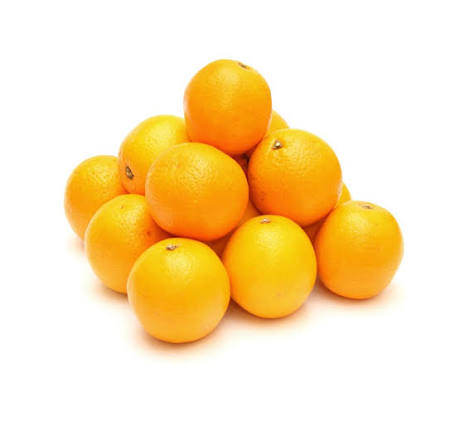
\includegraphics[width=4.5cm, trim={0cm 2cm 0cm 0cm}, clip]{images/oranges.jpeg}
            }
            \end{figure}
            \end{center}
        \item $n=2$ --- Фейеш Тот (1940);
        \item $n=3$ --- Хейлс, Фергюсон (1998--2005);
        \item $n>3$ --- сложная задача, есть лишь частичные результаты.
    \end{itemize}
    \note{
        \begin{itemize}
            \item Центры шаров образуют решётку, поиск плотных упаковок --- поиск решёток определённой очень хорошей структуры
            \item Даже в размерности 2 «очевидный» ответ (гексагональная упаковка) доказывается нетривиально: Лагранж закрыл только случай решёток, а полное доказательство для произвольных (не обязательно решётчатых) упаковок появилось только в 1940 году, после того как более ранняя попытка Туэ была признана неполной
            \item В размерности 3 доказательство заняло почти 400 лет и потребовало компьютера. Гипотеза Кеплера (1611), доказана Хейлсом (1998--2005)
        \end{itemize}
    }
\end{frame}

\begin{frame}{От решёток к упаковкам шаров}
    \begin{itemize}
        \item Обозначение: $\lambda_1(L)=\min_{\mathbf{v}\in L\setminus\{0\}}|\mathbf{v}|$ --- длина кратчайшего ненулевого вектора («первый минимум») решётки $L\subset\mathbb{R}^n$;
        \item Шары радиуса $\rho(L) = \tfrac12\lambda_1(L)$ с центрами в точках $L$ не пересекаются --- упаковка, отвечающая решётке $L$;
        \item Контактное число (kissing number) --- число ближайших соседей нуля:
        \[\tau(L) = \big|\{\mathbf{v}\in L : |\mathbf{v}|=\lambda_1(L)\}\big| = r_L(\lambda_1(L)^2)\]
        %  --- ;
        \item Примеры: 
        \begin{itemize}
        \item $\mathbb{Z}^n$: $\lambda_1=1$, $\tau=2n$;
        \item гексагональная: $\lambda_1=1$, $\tau=6$\\
        (или для $\sim\mathbf{A}_2$: $\lambda_1=\sqrt2$, $\tau=6$);
        \item $\mathbf{E}_8$: $\lambda_1=\sqrt2$, $\tau=240$.
        \end{itemize}
        \item Упаковки бывают нерешёточные: центры шаров образуют дискретное множество, но не обязательно группу; например, в $\mathbb{R}^{10}$ лучшая известная упаковка --- нерешёточная.
    \end{itemize}
    \note{
        \begin{itemize}
            \item Пусть $\overline B(0,r)\subset\mathbb{R}^n$ --- шар радиуса $r$, положим $\lambda_i(L)$ --- наименьшее $r$, при котором $L\cap\overline B(0,r)$ содержит $i$ линейно независимых векторов;
            \item $\lambda_1(L)\leq\lambda_2(L)\leq\dots\leq\lambda_n(L)$, $\lambda_i(L)$ --- «последовательные минимумы»;
        \end{itemize}
    }
\end{frame}

\begin{frame}{Ячейка Вороного}
    \begin{itemize}
        \item Ячейка Вороного решётки $L$:
        \[V(L) = \{\mathbf{x}\in\mathbb{R}^n : |\mathbf{x}|\leq|\mathbf{x}-\mathbf{v}|\ \forall\,\mathbf{v}\in L\}\]
        \item Примеры:
        \vspace{-1ex}
        \begin{center}
        \begin{figure}
        \captionsetup{justification=centering}
        \subcaptionbox*{$\mathbb{Z}^2$:\ \ $V(L)=[-\tfrac12,\tfrac12]^2$ (квадрат)}[5.5cm]{
            \begin{tikzpicture}[scale=0.9]
                \begin{scope}
                    \clip (-1.6,-1.6) rectangle (1.6,1.6);
                    \foreach \k in {-2,...,3}{
                        \draw[dashed] (\k-0.5,-2.5) -- (\k-0.5,2.5);
                        \draw[dashed] (-2.5,\k-0.5) -- (2.5,\k-0.5);
                    }
                    \fill[ThemeLight] (-0.5,-0.5) rectangle (0.5,0.5);
                    \draw[thick] (-0.5,-0.5) rectangle (0.5,0.5);
                    \foreach \i in {-2,...,2}{
                        \foreach \j in {-2,...,2}{
                            \fill (\i,\j) circle (2pt);
                        }
                    }
                \end{scope}
            \end{tikzpicture}
        }\hspace{0.6cm}%
        \subcaptionbox*{гексагональная:\ \ $V(L)$ --- правильный шестиугольник}[5.5cm]{
            \begin{tikzpicture}[scale=0.9]
                \begin{scope}
                    \clip (-1.8,-1.5) rectangle (1.8,1.5);
                    \foreach \i in {-3,...,3}{
                        \foreach \j in {-3,...,3}{
                            \draw[dashed] ({\i*1+\j*1/2+1/2},{\j*sqrt(3)/2+sqrt(3)/6}) -- ({\i*1+\j*1/2},{\j*sqrt(3)/2+sqrt(3)/3}) -- ({\i*1+\j*1/2-1/2},{\j*sqrt(3)/2+sqrt(3)/6}) -- ({\i*1+\j*1/2-1/2},{\j*sqrt(3)/2-sqrt(3)/6}) -- ({\i*1+\j*1/2},{\j*sqrt(3)/2-sqrt(3)/3}) -- ({\i*1+\j*1/2+1/2},{\j*sqrt(3)/2-sqrt(3)/6}) -- cycle;
                        }
                    }
                    \fill[ThemeLight] ({1/2},{sqrt(3)/6}) -- (0,{sqrt(3)/3}) -- ({-1/2},{sqrt(3)/6}) -- ({-1/2},{-sqrt(3)/6}) -- (0,{-sqrt(3)/3}) -- ({1/2},{-sqrt(3)/6}) -- cycle;
                    \draw[thick] ({1/2},{sqrt(3)/6}) -- (0,{sqrt(3)/3}) -- ({-1/2},{sqrt(3)/6}) -- ({-1/2},{-sqrt(3)/6}) -- (0,{-sqrt(3)/3}) -- ({1/2},{-sqrt(3)/6}) -- cycle;
                    \foreach \i in {-3,...,3}{
                        \foreach \j in {-3,...,3}{
                            \fill ({\i*1+\j*1/2},{\j*sqrt(3)/2}) circle (2pt);
                        }
                    }
                \end{scope}
            \end{tikzpicture}
        }
        \end{figure}
        \end{center}
        \item $V(L)$ --- фундаментальная область как и $P(L)$ (сдвиги $V(L)+\mathbf{v}$, $\mathbf{v}\in L$, замощают $\mathbb{R}^n$);
        \item $\mathrm{vol}(V(L))=\mathrm{vol}(P(L))=\mathrm{vol}(L)$.
    \end{itemize}
    \note{
        \begin{itemize}
            \item $V(L)$ --- выпуклый многогранник (пересечение полупространств, отвечающих серединным перпендикулярам к отрезкам до соседних точек $L$); в общем случае у него больше граней, чем у $P(L)$, но объём --- тот же $\mathrm{vol}(L)$.
        \end{itemize}
    }
\end{frame}

\begin{frame}{Упаковки и покрытия}
    \begin{itemize}
        \item Радиус упаковки $\rho(L)$ --- радиус наибольшего шара, вписанного в $V(L)$;
        \item Радиус покрытия $\mu(L)$ --- радиус наименьшего шара, содержащего $V(L)$;
        \item $\rho(L)\leq\mu(L)$
        \item Плотность упаковки: $\Delta(L) = V_n\,\rho(L)^n\,/\,\mathrm{vol}(L)$,\\ где $V_n=\pi^{n/2}/\Gamma(n/2+1)$ --- объём единичного шара в $\mathbb{R}^n$;
        \item Т.е. $\Delta(L)$ --- отношение объема вписанного шара к объёму ячейки Вороного;
        \item Плотность покрытия: $\Theta(L)=V_n\,\mu(L)^n/\mathrm{vol}(L)$;
        \item $\Delta(L) \leqslant 1 \leqslant \Theta(L)$
        \item Примеры:
        \[
        \begin{array}{c|ccccc}
        L & \rho & \mu & \mu/\rho & \Delta & \Theta\\\hline
        \mathbb{Z}^n & \frac12 & \frac{\sqrt n}2 & \sqrt n & V_n/2^n & V_n(\sqrt n/2)^n\\
        \mathbf{A}_2 & \frac1{\sqrt2} & \frac{\sqrt6}3 & \frac2{\sqrt3}\approx1.155 & \frac{\pi}{\sqrt{12}}\approx0.907 & \frac{2\pi}{3\sqrt3}\approx1.209\\
        \mathbf{E}_8 & \frac1{\sqrt2} & 1 & \sqrt2\approx1.414 & \frac{\pi^4}{384}\approx0.254 & \frac{\pi^4}{24}\approx4.059
        \end{array}
        \]
    \end{itemize}
    \note{
        \begin{itemize}
            \item $\Delta(L)$ не зависит от масштаба ($L\mapsto cL$ не меняет $\Delta$), в отличие от $\rho$, $\mathrm{vol}$ по отдельности --- удобный безразмерный инвариант подобия (ср. слайд «Изометрия и подобие»).
            \item Смысл $\mu(L)$: это худший случай при аппроксимации точки $\mathbb{R}^n$ ближайшей точкой решётки --- наибольшее возможное расстояние от произвольной точки пространства до ближайшего $\mathbf{v}\in L$ (радиус, гарантирующий покрытие всего $\mathbb{R}^n$ шарами вокруг точек $L$).
            \item Точки, реализующие $\mu(L)$ (вершины $V(L)$, наиболее удалённые от $\mathbf{0}$), называются глубокими дырами (deep holes) решётки; для $\mathbf{A}_2$ это центры треугольников решётки.
            \item Задача о наилучшем покрытии (минимизация $\Theta(L)$ по $L$) --- в некотором смысле двойственная к задаче об упаковке; решётка, оптимальная для одной задачи, не обязана быть оптимальной для другой (известные примеры расхождения при больших $n$).
        \end{itemize}
    }
\end{frame}

\begin{frame}{Максимальная плотность}
    \begin{itemize}
        \item Теорема (Минковский--Хлавка, 1943): для любого $n\geqslant2$ существует решётка $L\subset\mathbb{R}^n$ с $\Delta(L)\ \geqslant\ \dfrac{\zeta(n)}{2^{\,n-1}}$, где $\zeta$ --- дзета-функция Римана;
        \item Пусть $\Delta_n$ --- максимально возможная плотность упаковки шаров в $\mathbb{R}^n$ (по всем упаковкам, не только решёточным);
        \item $\Rightarrow$ $\Delta_n\geqslant\zeta(n)\,2^{1-n}$;
        \item Точное значение $\Delta_n$ известно лишь для $1,2,3,8,24$;
        \item Во всех известных случаях $\Delta_n$ достигается на решётке ($\mathbb{Z}$, $\mathbf A_2$, $\mathbf E_8$, решётка Лича).
    \end{itemize}
    \note{
        \begin{itemize}
            \item $\Delta_n\geqslant\zeta(n)\,2^{1-n}$ --- по сей день лучшая известная асимптотика по порядку роста;
            \item  кроме $n=3$, где та же плотность реализуется ещё и нерешёточной упаковкой: гексагональная плотноупакованная упаковка (ГПУ или HCP) --- упаковка слоями $ABAB\dots$ (третий слой над первым), в отличие от гранецентрированная кубическая (ГЦК или FCC) со слоями $ABCABC\dots$; та же плотность $\pi/\sqrt{18}$, но ГПУ --- не решётка.
        \end{itemize}
    }
\end{frame}

\begin{frame}{Модулярность и плотность}
    \begin{itemize}
        \item Метод Кона--Элкиса (2003): верхняя граница на плотность упаковки шаров --- бесконечномерная LP над классом функций $f$:
        \begin{itemize}[<.->]
            \item если $f:\mathbb{R}^n \to \mathbb{R}$ --- такая, что
            \[
            \begin{gathered}
            f(x)\leqslant 0\ \text{при } |x|\geqslant 2\rho,\quad \hat f(y)\geqslant 0\ \forall y\in \mathbb{R}^n\\[-0.3ex]
            {\small (\,\hat f\ \text{--- преобр. Фурье;}\ f,\hat f\ \text{интегрируемы, с достаточным запасом убывания на }\infty\,)}
            \end{gathered}
            \]
            \item то для $\Delta_n$ --- плотности упаковки шаров радиуса $\rho$ (ср. $\rho(L)$ выше):
            \[\Delta_n \leqslant V_n\,\rho^{n}\,\frac{f(0)}{\hat f(0)},\qquad V_n=\frac{\pi^{n/2}}{\Gamma(n/2+1)};\]
        \end{itemize}
        \item $\Rightarrow$ Найти плотную упаковку в $\mathbb{R}^n$ $\leftrightsquigarrow$ Предъявить функцию-сертификат $f$.
        \item Размерности $8$ и $24$ (Вязовская et al., 2016--2017): такие функции найдены за счет свойств симметрий квазимодулярных функций при $z\mapsto -1/z$.
    \end{itemize}

    \note{
        \begin{itemize}
            \item Суть метода Кона–Элкиса — свести геометрическую комбинаторную задачу к поиску «магической» функции с нужными свойствами по обе стороны преобразования Фурье; существование такой функции автоматически даёт верхнюю оценку плотности, а удачный выбор функции может дать и точный ответ.
            \item Технически на $f$ нужны условия допустимости (integrable + decay, напр. Schwartz-класс или $|f(x)|,|\hat f(x)|\lesssim (1+|x|)^{-n-\varepsilon}$) --- без этого сумма/формула Пуассона, на которой всё держится, просто не сходится;
        \end{itemize}
    }
\end{frame}

% ============================================================
\section{В сторону приложений}
% ============================================================

\begin{frame}{Решётки в теории кодирования}
    \begin{itemize}
        \item Передача данных по каналу с гауссовским шумом:
        \vspace{1ex}
        \begin{center}
            \begin{tikzpicture}[every node/.style={font=\footnotesize}, box/.style={draw, rounded corners, minimum height=1.3cm, minimum width=2.8cm, align=center}, >=stealth]

                \node[box] (src)  at (0,1)   {Сигнал $f(t)$};
                \node[box] (samp) at (3.4,1) {Семплирование\\ $f(t) \mapsto \mathbf x\in\mathbb R^n$};
                \node[box] (enc)  at (6.8,1) {Кодирование\\(квантование)\\ $\mathbf x\mapsto\mathbf c\in L$};
                \node[box] (tx)   at (10.2,1) {Передача\\в канал};

                \draw[->] (src)  -- (samp);
                \draw[->] (samp) -- node[above]{$\mathbf x$} (enc);
                \draw[->] (enc)  -- node[above]{$\mathbf c$} (tx);

                \node[box] (rx)   at (10.2,-1.5) {Получение\\из канала};
                \node[box] (dec)  at (6.8,-1.5) {Декодирование\\ $\arg\min\limits_{\mathbf v\in L}|\mathbf r-\mathbf v|$};
                \node[box, minimum width=6.2cm] (gen)  at (1.7,-1.5) {Генерация сигнала};

                \draw[->, decorate, decoration={snake, amplitude=1mm, segment length=4mm, post length=2mm}] (tx) -- node[right, align=left]{$\mathbf r = \mathbf c + \mathbf e$\\ (шум)} (rx);
                \draw[->] (rx)  -- node[above]{$\mathbf r$} (dec);
                \draw[->] (dec) -- node[above]{$\hat{\mathbf c}$} (gen);
            \end{tikzpicture}%
        \end{center}
        \item Если $|\mathbf e|<\rho(L)$, то декодирование гарантированно верно;
        \item Ошибки декодирования связаны с контактным числом $\tau(L)$;
        \item Ошибка квантования контролируется радиусом покрытия $\mu(L)$;
        \item $\Rightarrow$ чем плотнее упаковка, тем лучше код.
    \end{itemize}
    \note{
        \begin{itemize}
            \item Условие $|\mathbf e|<\rho(L)$ --- лишь достаточное: шум, вышедший за пределы вписанного шара, но оставшийся внутри самой ячейки Вороного точки $\mathbf c$, всё ещё декодируется верно; ошибка возможна, только когда $\mathbf r$ покидает ячейку Вороного $\mathbf c$.
            \item Полный выигрыш решёточного кода раскладывается на два независимых слагаемых: coding gain --- от плотности самой решётки $\Delta(L)$ (это и есть наша задача про упаковки), и shaping gain --- от формы конечной кодовой книги (подмножества точек $L$ с ограничением на среднюю энергию, например шар вместо куба).
            \item Эрез--Замир (Erez--Zamir, 2004) показали, что решётки с надлежащим декодированием (MMSE lattice decoding) асимптотически ($n\to\infty$) достигают пропускной способности AWGN-канала --- то есть хорошие решётки не просто уменьшают вероятность ошибки, а решают задачу оптимального кодирования целиком.
        \end{itemize}
    }
\end{frame}

\begin{frame}{Решётки в криптографии}
    \begin{itemize}
        \item Задача декодирования --- найти вектор $L$ ближайший к заданной точке --- Closest Vector Problem (CVP);
        \item Shortest Vector Problem (SVP): найти кратчайший ненулевой вектор в $L$;
        \item Что если решётка задана «плохим» базисом?
        \vspace{1ex}
        \begin{center}
        \begin{figure}
        \captionsetup{justification=centering}
        \subcaptionbox*{$\mathbf{v}_1=(\frac32,0)$, $\mathbf{v}_2=(\frac12,\frac54)$\\ «хороший» базис}{
            \begin{tikzpicture}[scale=0.55]
                    \foreach \i in {-1,...,3}{
                        \foreach \j in {0,...,3}{
                            \fill ({\i*3/2 + \j*1/2},{\j*5/4}) circle (2pt);
                        }
                    }
                \draw[-{Stealth[length=2mm]}, thick] (0,0) -- (3/2,0);
                \draw[-{Stealth[length=2mm]}, thick] (0,0) -- (1/2,5/4);
            \end{tikzpicture}
        }\hspace{1.2cm}%
        \subcaptionbox*{$\mathbf{v}_1'=(\frac{11}{2},\frac52)$, $\mathbf{v}_2'=(\frac72,\frac54)$\\ «плохой» базис}{
            \begin{tikzpicture}[scale=0.55]
                    \foreach \i in {-1,...,3}{
                        \foreach \j in {0,...,3}{
                            \fill ({\i*3/2 + \j*1/2},{\j*5/4}) circle (2pt);
                        }
                    }
                \draw[-{Stealth[length=2mm]}, thick] (0,0) -- (11/2,5/2);
                \draw[-{Stealth[length=2mm]}, thick] (0,0) -- (7/2,5/4);
            \end{tikzpicture}
        }
        \end{figure}
        \end{center}
        \item SVP, CVP --- вычислительно сложные (NP-трудные) задачи, основа криптографических схем.
    \end{itemize}
    \note{
        \begin{itemize}
            \item Интуиция: например в SVP/CVP трудность задач зависит от качества базиса --- плохой базис прячет короткие векторы.
            \item Другие задачи, например: Lattice Isomorphism Problem (LIP)
            \item LLL (Ленстра--Ленстра--Ловас, 1982) --- полиномиальный алгоритм, превращающий «плохой» базис в «приведённый» (почти ортогональный), с гарантией на длину найденного вектора $\|b_1\|\le 2^{(n-1)/4}\lambda_1(L)$ --- не решает SVP/CVP точно, но даёт эффективную аппроксимацию.
        \end{itemize}
    }
\end{frame}

\begin{frame}{Решётки в математической оптимизации}
    \begin{itemize}
        \item Целочисленное программирование (IP): пусть $A\in\mathbb{Z}^{m\times n}$, $\mathbf{b}\in\mathbb{Z}^m$, найти
        \[\mathbf{x}\in\mathbb{Z}^n : A\mathbf{x}\le \mathbf{b}\]
        \item IP --- вычислительно сложная (NP-трудная) задача в общем случае.
        \item Теорема (Ленстра, 1983): при фиксированной размерности $n$ IP решается за полиномиальное время. (!! алгоритм экспоненциален по $n$)
        \item IP: сколько целых точек в выпуклом многограннике $P\subset\mathbb{R}^n$?
        \item Ещё один пример производящей функции:
            \[f_P(x_1,\dots,x_n) = \sum_{(v_1,\dots,v_n)\in P\cap\mathbb{Z}^n} x_1^{v_1}x_2^{v_2}\cdots x_n^{v_n};\]
        \item Теорема (Барвинок, 1994): При фиксированной размерности $n$ функция $f_P$ представима как короткая сумма рациональных функций и вычисляется за полиномиальное время. (!! число конусов в разбиении растёт экспоненциально по $n$)
    \end{itemize}
    \note{
        \begin{itemize}
            \item Схема доказательства теоремы Ленстры: Теорема о плоскостности (flatness theorem): «если выпуклое тело не содержит целых точек, то существует направление, вдоль которого это тело узкое»; Алгоритм LLL; $\Rightarrow$ достаточно перебрать полиномиально много «слоёв»;
            \item Схема доказательства теоремы Барвинока: Разбиение многогранника $P$ на симплициальные конусы; Производящая функция каждого конуса --- рациональная;
        \end{itemize}
    }
\end{frame}

\begin{frame}{Решётки и оптимальный дизайн эксперимента}
    \begin{itemize}
        \item Задача оптимального планирования эксперимента (DoE):
        \begin{center}
            Выбрать точки наблюдений $\mathbf{x}_1,\dots,\mathbf{x}_k \in \mathbb{R}^n$ так,\\ чтобы как можно точнее оценить параметры модели $y\sim f(\mathbf{x})$;
        \end{center}
        \item Для многих постановок DoE:
        \begin{center}
            Оптимальный план $\leftrightsquigarrow$ Плотные евклидовы/сферические упаковки;
        \end{center}
        \item Максиминный план с низкой дискрепантностью (Хэ, 2017): решётка с наилучшим известным радиусом покрытия $\to$ масштабирование/поворот/обрезка под область эксперимента;
        \item Программа Gosset (Хардин--Слоун, 1995): оптимальные планы экспериментов на базе конструкций упаковок/сферических кодов.
    \end{itemize}

    \note{
        \begin{itemize}
            \item Дизайн эксперимента (design of experiments, DOE) --- классический раздел математической статистики, обычно у него нет ничего общего с решётками на первый взгляд.
            \item Мотив D-оптимальности --- максимально «растянуть» облако точек наблюдений, чтобы минимизировать дисперсию оценок --- отсюда естественная связь с равномерным покрытием сферы.
            \item Gosset --- практическая реализация этой идеи: тот же код/решётка, что даёт хорошую упаковку шаров или хороший корректирующий код, конвертируется в конкретный план эксперимента; см. также статью Hardin--Sloane, \textit{Codes (Spherical) and Designs (Experimental)} (1995), где эта параллель проведена явно.
            \item Xu He \textit{Rotated Sphere Packing Designs} : мотивация --- классический критерий maximin distance design (Johnson--Moore--Ylvisaker, 1990) --- расставить $n$ точек в кубе так, чтобы минимальное попарное расстояние было максимальным; это буквально задача упаковки шаров (точки --- центры непересекающихся шаров радиуса $r$, максимизировать $r$).
            \item Идея: вместо решения NP-трудной комбинаторной задачи заново для каждого $n$, $p$ (как в LHS / simulated annealing подходах) --- взять уже известную асимптотически оптимальную решётку (из таблиц Конвея--Слоуна), промасштабировать, повернуть и вырезать нужное число точек внутри куба.
            \item Зачем поворот: решётка бесконечна и не подогнана под границы куба --- без оптимального поворота возникают краевые артефакты и плохая проективная структура (важно, когда не все факторы существенны).
            \item Результат: design одновременно близок к оптимальному по maximin distance, имеет низкую дискрепантность (полезно для численного интегрирования) и хорошую проективную равномерность --- три классические цели DOE решаются одним геометрическим объектом.
            \item Общий мотив раздела: решётки --- на удивление универсальный язык для формулировки «максимально равномерно/эффективно расположить точки», от криптографии до статистики; тот же паттерн «хороший базис решётки $\Rightarrow$ решение прикладной задачи», что мы видели в алгоритме Ленстры и атаке Лагариаса--Одлыжко.
        \end{itemize}
    }
\end{frame}

% ================================================================
\begin{frame}{Итоги лекции}
    \begin{itemize}
        \item Решётка --- пример $\mathbb{Z}$-модуля; модули над кольцами --- еще одна важная алгебраическая структура;
        \item Неприводимые решётки и разложение на неприводимые --- аналогия с простыми числам;
        \item Математические объекты можно изучать через их характеристики и инварианты (относительно некоторого преобразования/воздействия);
        \item Тета-функция решётки --- пример инвариант с «богатым внутренним миром» (модулярность);
        \item В следующий раз --- группы, их действия и представления.
    \end{itemize}
\end{frame}
\note{%
\begin{itemize}
    \item ---
\end{itemize}
}

% ================================================================
% \begin{frame}{Литература}
%     \begin{itemize}[<.->]
%         \item TODO источники по решеткам
%         \item W. Stein, \textit{Modular Forms: A Computational Approach}\\ --- мягкий вход в МФ, с вычислениями в SageMath;
%         \item W. Ebeling, \textit{Lattices and Codes}\\ --- изложение с точки зрения приложений к кодам;
%         \item N. Koblitz, \textit{Introduction to Elliptic Curves and Modular Forms,} (есть перевод)\\ --- классический мост между ЭК и МФ;
%         \item D. Zagier et al., \textit{The 1-2-3 of Modular Forms}\\ --- более широкий контекст МФ и приложений;
%     \end{itemize}
% \end{frame}
% \note{%
% \begin{itemize}
%     \item Всё, что было показано без доказательств, разбирается подробно в источниках выше; полное строгое изложение --- в отдельном курсе алгебраической теории чисел (A-I).
% \end{itemize}
% }

\end{document}